\chapter{Grundlagen, Analyse von Use Cases zur Dokument\"ahnlichkeitsbestimmung }
\label{chap:Grundlagen}

In this chapter we give an explanation about the technologies and concepts this diploma thesis relies on. We start describing the fundamental concepts and introduce the components and prototypes that form the basis of our work.

\section{Informationsrückgewinnung}
\label{sec:Informationsrückgewinnung}

In the last decades our world has become more and more interconnected. This interconnection added to the increase of the available bandwidth and the change in business models have forced IT Systems to fulfill its demands, leading to its reorganization into a public utility which offers public services, like water, electricity, etc. The \ac{NIST} defines Cloud computing as "a model for enabling ubiquitous, convenient, on-demand network access to a shared pool of configurable computing resources (e.g., networks, servers, storage, applications, and services) that can be rapidly provisioned and released with minimal management effort or service provider interaction"  \cite{NIST2011}. The Cloud computing model is composed of five characteristics:
	\begin{enumerate}
		\item On-demand self-service: a Cloud user consumes the Cloud provider's computing capabilities automatically without the need of human interaction. 
		\item Broad network access: computing capabilities are available via the network and can be accessed using standard mechanisms.
		\item Resource pooling: computing capabilities in the Cloud provider side are virtualized to serve multiple consumers simultaneously using a multi-tenant model. The Cloud consumer generally has no sense of the provided resources.
		\item Rapid Elasticity: computing and storage resources can be dynamically (and in some cases automatically) provisioned and released to respond to the actual consumers' demand.
		\item Measured Service: resources' usage is monitored and measured in a transparent way to the Cloud consumer and provider for control and optimization purposes.
	\end{enumerate}

The control that the Cloud consumer has over the computer resources in a Cloud provider infrastructure is defined in three service models: \term{\ac{SaaS}}, \term{Platform-as-a-Service (\ac{PaaS})} and \term{\ac{IaaS}}. \term{\ac{SaaS}} provides to the Cloud consumer access and usage of Cloud provider's applications running on a Cloud infrastructure. The consumer has no control over the underlying infrastructure where the application he uses is deployed. The customer can only control individual application's configurations during his usage of it. \term{\ac{PaaS}} provides the customer with the needed capabilities to deploy applications which's programming language, required libraries, services and tools are supported by the provider. The consumer has no control over the underlying infrastructure where he deploys the application. \term{\ac{IaaS}} is the model which gives most control to the consumer. Thus, the consumer is able to deploy and run arbitrary software and has the control over operating systems, storage and deployed applications, but has no management or control on the underlaying Cloud infrastructure. 

Although the three service models described above provide both data computation and storage capabilities for the consumer, they do not provide to the customer the possibility to directly and uniquely purchase access of storage services. In this diploma thesis we concentrate in two concrete models: \term{\ac{DBaaS}} and \term{\ac{STaaS}}. Cloud storage providers target a selected number of consumers, who process their data on-premise, but do not  want to cover the expenses of a local database system, or a backup system, among others. The Cloud storage model alleviates the need in organizations to invest in database hardware and software, to deal with software upgrades, and to maintain a professional team for its support and maintenance \cite{dbaasIyer}.  \ac{DBaaS} and \ac{STaaS} can be considered quite similar, except for one of their main distinction characteristics: their access interface. The former is the most robust data solution offered as a service, as it offers a full-blown database functionality. It can be accessed via the most common database protocols, such us MySQL, Oracle, etc, or by REST interfaces supporting \ac{SQL}. Examples of this model are Amazon RDS \cite{amazonrds} and Oracle Cloud \cite{oraclecloud}. On the other hand, the latter provides REST, \ac{SOAP} over \ac{HTTP}, or Web-based interfaces in order to perform the operations over the stored data \cite{cloudstorageWU}. Examples of this model are Amazon Dynamo \cite{amazondynamodb} , Google App Engine Datastore \cite{googleappdatastore}, and Dropbox \cite{dropbox}.

\ac{NIST} defines four deployment models in Cloud computing. A private Cloud consists in a Cloud infrastructure which is provisioned exclusively for one organization and used by the members conforming the organization. It is comparable to processing facilities that are enhanced with the Cloud computing characteristics. A community Cloud is a Cloud infrastructure where its use is limited to organizations which share the same requirements. A public Cloud infrastructure can be accessed and used by the public. It is usually offered by Cloud service providers that sell Cloud services made for general public or enterprises. Some of the Cloud consumers may process and store information which requires more control over the infrastructure in which is located, or consume public Cloud computing resources during peak loads in their private Cloud infrastructure. The hybrid Cloud model combines two or more deployment models described above and the combination remains as a unique entity.  

Cloud computing and \ac{SOA} are related styles at an architectural, solution and service level, according to IBM \cite{IBM2011}. Cloud providers expose their Cloud infrastructure as services as part of a \ac{SOA} solutions and the communication between Clouds in the Hybrid Cloud model described above can be compared to a SOA communication solution between enterprises. Cloud services are services that can be accessed by the Cloud consumers through the network. Therefore, we can deduce that the SOA model can be applied in the Cloud computing approach. As the \ac{ESB} is the central piece of \ac{SOA}, the need of the \ac{ESB} in a Cloud computing infrastructure as an integration middleware for the Cloud services is essential. 
\section{Grundlagen der Bayesschen Statistik}
\label{sec:BayesscheStatistik}  

%Weerawarana et al. define SOA as an specific architectural style that is concerned with loose coupling and dynamic binding between services \cite{Weera2005}.

%In the last years communication between external components whose functionalities are exposed as services has been a hard task when there was not previous agreement on message protocols, data types and encoding, and used middleware technology. Due to the economic and technological growth needed, enterprises had to adapt the \ac{SOA} paradigm in their existing IT Infrastructure. \ac{SOA} provides the needed flexibility by building an architectural style with the following benefits: loose coupling, interoperability, efficiency, and standardization. The W3C group defines SOA as a form of distributed system architecture that is typically characterized by the following properties \cite{w3csoa}:
%	\begin{itemize}
%		\item Logical view: the service's functionality is exposed, but not its internal logic.
%		\item Message orientation: the internal structure of an agent is abstracted.
%		\item Description orientation: a service is described by machine-processable meta data.
%		\item Granularity: services tend to use a small number of operations with relatively large and complex messages.
%		\item Network orientation: Services tend to be oriented toward use over a network.
%		\item Platform neutral: Messages are sent in a platform-neutral, standardized format delivered through the interfaces.
%	\end{itemize}

%\ac{SOA} defines three main roles: requester, provider and broker and the four main operations: publish, find, bind, and invoke. The service provider provides access to services, creates a description of a service and publishes it to the service broker. The service requestor discovers a service by searching through the service descriptions located in the service broker. When the service which best fits to his needs is found, the discovering facility provides the concrete service endpoint and the consumer is responsible for binding to it.  With this information, the requestor can then bind to the concrete service and finally execute a business activity \cite{Weera2005}. The service broker provides support for service registration and binding. 

%The main component in a \ac{SOA} is the \ac{ESB}. The functionalities provided by a service bus can simplify the process (publication, discovery, binding, and invocation) and make it more transparent to provide an ease-to-use experience for a Web service based implementation of \ac{SOA} \cite{Weera2005}. Chappel defines its function as an intermediate connection provisioning of service providers with service consumers and thereby ensure decoupling of theses \cite{Chapp2004}. 

\subsection{Definition und Hintergrund}
\subsection{Anwendungsgebiete und Nutzen}
\subsection{Modelle, Parameter und Überzeugungen}
\subsection{Die Wahrscheinlichkeit}
\subsection{Der Satz von Bayes}
%The flow of data and information is a key for driving business decisions in IT organizations \cite{Chapp2004}. Furthermore, the interaction between loosely coupled components within an organization or with third party organizations requires distributed systems mechanisms which provide communication support for different protocols, and reliability. SOA has fulfilled this main requirement by providing an integration environment with minimal (or any) integration efforts. 

%The \ac{ESB} is the central component in \ac{SOA}. It provides a loosely coupled, event-driven \ac{SOA} with a highly distributed universe of named routing destinations across a multi-protocol message bus \cite{Chapp2004}. An \ac{ESB} provides an abstract decoupling between connected applications by creating logical endpoints which are exposed as services and conform a multi-protocol environment, where routing and data transformation are transparent to the service connected to it. Furthermore, when using an \ac{ESB}, in the first place, services are configured rather than coded, demanding minimal adaptation, implementation and maintenance efforts. The programmer just has to implement the binding to the logical endpoint exposed as a service. In the second place, \ac{ESB} routing is based on a reliable messaging router. Applications don't need to include message system-failure forwarding mechanisms, to know which data formats are needed in the consumed services, or to care about future changes in applications or services the applications interact with. An \ac{ESB} hides the complexity of orchestration between services in business processes. 

%Chappel defines the combination of loosely coupled interfaces and asynchronous interactions as a key concept of the bus terminology  \cite{Chapp2004}. A user of the bus can access every service registered in the bus. For this purpose, it implements the \ac{SOA} operations in order to make them transparent to the user who can therefore focus on: plugging to the bus and posting and receiving data from the bus. Furthermore, the \ac{ESB} can form the core of a pervasive grid \cite{Chapp2004}. Services supported by an organization can be organized between the \ac{ESB}s conforming the grid, as well as its access between the organizational departments, and services provided to third party organizations. 

%\begin{figure}[htb]
%	\centering
%		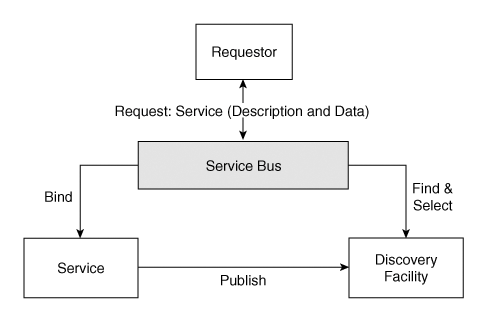
\includegraphics[clip, scale=0.7]{./gfx/servicebus.png}
%	\caption[The Role of the service bus in SOA]{The Role of the service bus in \ac{SOA} \cite{Weera2005} }
%	\label{fig:servicebus}
%\end{figure}

%(see Figure \ref{fig:servicebus})

%When receiving a service description (\ac{WSDL}) and data from the service requester, the \ac{ESB} is responsible for selecting the service which best fits to the description requirements, for binding the service requester with the backend service through a route created between the logical endpoints and for making the necessary data transformations to enable the communication between the parts.

%As the \ac{ESB} is the central component in \ac{SOA}, and established as integration middleware for services, in this diploma thesis we focus on the required modifications and extensions in the open-source \ac{ESB} Apache ServiceMix 4.3 to provide transparent communication support between the applications and its data located in on-premise databases, or migrated to off-premise data stores. 

%\FloatBarrier
\section{Analyse von Use Cases für die Dokumentähnlichkeitsbestimmung}
\label{sec:AnalyseUse}   

One of the main decision variables for utilizing a Cloud computing environment are capital expenditures. The main goal of a Cloud consumer is to minimize its business costs when migrating to the Cloud. According to Chong, a \ac{SaaS} solution benefits a Cloud customer with the following advantages \cite{ChongB2006}:

	\begin{itemize}
		\item The Cloud consumer does not directly purchase a software license, but a subscription to the software offered as a service by the Cloud infrastructure. 
		\item More than half of the IT investments of a company are made in infrastructure and its maintenance. In a \ac{SaaS} solution this responsibilities are mainly externalized to the Cloud provider.   
		\item A Cloud computing environment is based on the utilization of its resources simultaneously by a large number of Cloud consumers. For example, a Cloud provider that offers a centrally-hosted software service to a large number of customers can serve all of them in a consolidated environment and lower the customer software subscription costs while maintaining or lowering the provider's infrastructure, administration and maintenance costs. 
		\item The cost leverage in the software utilization allows the Cloud providers to focus not only on big enterprises capable of large IT budgets, but also on the small business that need access to IT solutions. 
	\end{itemize} 

Multi-tenancy in a \ac{SaaS} environment allows the Cloud providers to lower the cost per customer by optimizing the resources usage in the Cloud infrastructure. The software serves multiple tenants concurrently, who share the same code base and data storage systems. Chong and Carraro \cite{ChongB2006} define a well designed \ac{SaaS} application as scalable, multi-tenant-efficient and configurable. With this design patterns, the \ac{SaaS} model enables the provider to \term{catch the long tail}. Business softwares are becoming more complex and tend to demand an individual customer support and an increase of the computing and storage resources in the infrastructure. This fact leads to an increase in the infrastructure investment and maintenance costs. However, if the previous requirements are eliminated and the provider's infrastructure is scaled to combine and centralize customers' hardware and services requirements, the price reduction limit can be decreased and, in effect, allow a wide range of consumers to be able to access this services.

The reasons discussed above are also applicable in the \ac{DBaaS} and \ac{STaaS} models. Storage and retrieval of data involve high maintenance and management costs. The data management cost is estimated to be between 5 to 10 times higher than the data gain cost \cite{multishares2011}. Furthermore, storing data on-premise does not only require storing and retrieving data, but also requires dealing with disaster recovery, \ac{DBMS}, capacity planning, etc. Most of the organizations prefer to lead their investments to their local business applications rather than becoming a data management company \cite{multishares2011}. Cloud storage providers offer a pay-per-use storage model, e.g. based on storage capacity or based on number of connections to the storage system, and ensure that the stored data will persist over time and its access through the network. However, security and confidentiality are the main constraints when moving private data to a shared public infrastructure. 

\begin{figure}[htb]
	\centering
		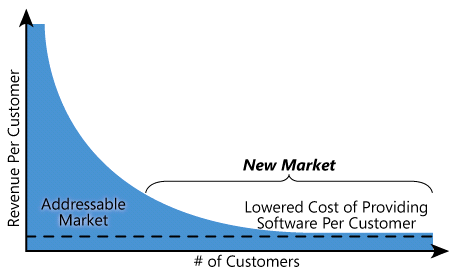
\includegraphics[clip, scale=0.5]{./gfx/longtail.png}
	\caption[Multi-tenancy and Long Tail]{New market opened by lower cost of SaaS \cite{ChongB2006}}
	\label{fig:longtail}
\end{figure}

In the Figure \ref{fig:longtail} the economics of scaling up to a high number of customers while reducing the software price is analyzed. Cloud providers have reached a new market formed by small or medium businesses without enough budget for building an on-premise IT infrastructure.

Multi-tenancy refers to the sharing of the whole technological stack (hardware, operating system, middleware, and application instances) at the same time by different tenants and their corresponding users \cite{EnablingMT}. Andrikopoulos et al. identify two fundamental aspects in multi-tenant awareness: communication, and administration and management \cite{andrikopoulos2013}. The former involves isolated message exchanges between tenants and the latter allows tenants individual configuration and management of their communication endpoints. Utilizing an \ac{ESB} as the central piece of communication middleware between applications in a \ac{PaaS} environment forces it to ensure multi-tenancy at both communication, and administration and management, as mentioned before. The multi-tenancy support modifications made in the open-source ServiceMix 4.3 are the results of \cite{Essl2011}, \cite{Muhler2012}, and \cite{gomez2012}. In this diploma thesis we reuse and extend those results in oder to provide multi-tenant transparent Cloud data access in the Cloud through the \ac{ESB}, when the application's data is migrated and accessed through the \ac{ESB} in a Cloud infrastructure.

The migration of an application's stack to the Cloud can be done at different levels of the application's stack: Presentation Layer, Business Layer, and Data Access Layer. The Replacements of Components with Cloud offerings migration type is the least invasive type of migration \cite{andrikopoulos2013}. In this diploma thesis we focus on this type of migration, concretely when the used Cloud offering is the database system. Migration of the data can be either seen as the migration of the Data Layer (Data Access Layer and Database Layer) or of the whole application \cite{andrikopoulos2013}. Migration of the Data Layer to the Cloud means migrating the both data management and data access to the Cloud, while maintaining its transparency to the application's Business Layer. 

In a Cloud infrastructure where Cloud storage is offered, Feresten identifies four main tenant requirements: security, performance, data protection and availability, and data management \cite{feresten2010}. Multi-tenancy in a storage system can be achieved by aggregating tenant-aware meta-data to the tenant's data (see Figure \ref{fig:virtualstoragecontainer}), or by physical storage partitioning, but this is not sufficient when fulfilling the data management, and the flexibility requirement. Tenants must have independent access and management, as if they accessed their own data storage systems. For this purpose, storage vendors have introduced the concept of \term{virtual storage container}, a tenant-aware management domain which grants all (or most of) the database management operations over the storage container, as described in Figure \ref{fig:virtualstoragecontainer}.

\begin{figure}[htb]
	\centering
		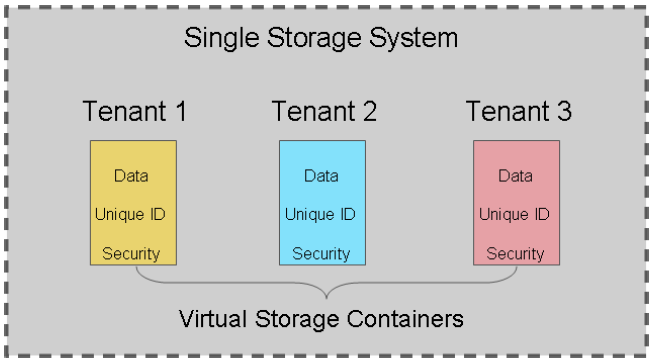
\includegraphics[clip, scale=0.4]{./gfx/virtualstoragecontainer.png}
	\caption[Virtual Storage Container]{Attributes of a Virtual Storage Container \cite{feresten2010}}
	\label{fig:virtualstoragecontainer}
\end{figure}

In this diploma thesis we must take into account the different approaches that most of the Cloud storage vendors have taken into account, in order to provide the tenant transparent access through the \ac{ESB} to his virtual storage container in one or more Cloud infrastructures.

\subsection{Finden von Dokumenten mit ähnlichen Inhalten(Duplikaten Findung)}
\subsection{Verwendung von a priori Wissen}
\subsection{Systemübergreifende „Fremdschlüssel"}
\subsection{Profil Matching}
\subsection{Email Klassifikation (Spamfilter)}
\input{fundamentals/AnalyseAnsätze}
